% =====================================================================
%  SoCal Wildfires -- Grid Co-Simulation
%  Onboarding deck for graduate students new to the project
%
%  Project : https://gitlab.com/arl-experiments/socal-wildfires
%  Theme   : Cal State LA (gold + black, Montserrat / Open Sans)
%
%  Compile (preferred, for authentic brand typography):
%      xelatex socal-wildfires.tex && xelatex socal-wildfires.tex
%  Fallback:
%      pdflatex socal-wildfires.tex && pdflatex socal-wildfires.tex
% =====================================================================
\documentclass[aspectratio=169,9pt]{beamer}

\usetheme{CalStateLA}

\usepackage[english]{babel}
\usepackage{booktabs}
\usepackage{array}
\usepackage{amsmath}
\usepackage{etoolbox}
\usepackage{tikz}
\usetikzlibrary{arrows.meta,positioning,fit,backgrounds,shapes.geometric}

% --- Density tuning -----------------------------------------------------
% The theme is built for a 4:3 lecture deck with generous leading. This is a
% denser 16:9 briefing deck, so the leading, frame-title size and list/block
% spacing are all tightened to fit the content on one frame each.
\linespread{1.0}
\setbeamerfont{frametitle}{series=\bfseries, size=\large}
\setbeamerfont{framesubtitle}{series=\mdseries, size=\small}
\setbeamerfont{block title}{series=\bfseries, size=\small}
\setbeamerfont{block body}{size=\small}

\newcommand{\tightspacing}{%
  \setlength{\itemsep}{1.5pt}%
  \setlength{\parskip}{0pt}%
  \setlength{\parsep}{0pt}%
  \setlength{\topsep}{1.5pt}%
  \setlength{\partopsep}{0pt}%
}
\AtBeginEnvironment{itemize}{\tightspacing}
\AtBeginEnvironment{enumerate}{\tightspacing}
\AtBeginEnvironment{description}{\tightspacing}

% Trim the vertical padding beamer puts around blocks.
\addtobeamertemplate{block begin}{\vskip-2pt}{\vskip-1pt}
\addtobeamertemplate{block end}{\vskip-2pt}{\vskip1pt}
\addtobeamertemplate{block alerted begin}{\vskip-2pt}{\vskip-1pt}
\addtobeamertemplate{block alerted end}{\vskip-2pt}{\vskip1pt}

% --- Theme template overrides -------------------------------------------
% The shipped theme sizes its frametitle/footline boxes as
%   wd=\paperwidth + leftskip + rightskip
% which overflows every frame by 0.14\paperwidth. Both templates are
% restated here with the content width computed correctly, and the footer
% label is changed from the theme's course label to this deck's label.
\newlength{\csladeckinner}
\setlength{\csladeckinner}{\dimexpr\paperwidth-0.14\paperwidth\relax}

\makeatletter
% Frame title is typeset inside the text block, so content sits at
% \textwidth and only the full-bleed gold rule reaches back into the margin.
\setbeamertemplate{frametitle}{%
  \nointerlineskip%
  \makebox[0pt][l]{\hspace*{-\beamer@leftmargin}%
    \color{cslagold}\rule{\paperwidth}{3.5pt}}\par%
  \vskip3pt%
  {\usebeamerfont{frametitle}\usebeamercolor[fg]{frametitle}%
   \raggedright\insertframetitle\par}%
  \ifx\insertframesubtitle\@empty\else%
    \vskip1pt%
    {\usebeamerfont{framesubtitle}\usebeamercolor[fg]{framesubtitle}%
     \raggedright\insertframesubtitle\par}%
  \fi%
  \vskip2pt%
  {\color{csladarkgray}\rule{\textwidth}{0.5pt}}\par%
  \vskip2pt%
}
\makeatother

% Footer is typeset at \paperwidth, with the deck label in place of the
% theme's course label.
\setbeamertemplate{footline}{%
  {\color{cslagold}\rule{\paperwidth}{2pt}}\par%
  \vskip2pt%
  \hbox to\paperwidth{%
    \hspace*{0.07\paperwidth}%
    \usebeamerfont{footline}\color{csladarkgray}%
    SoCal Wildfires\,\textbar\,Grid Co-Simulation%
    \hfill%
    \insertframenumber\,/\,\inserttotalframenumber%
    \hspace*{0.07\paperwidth}%
  }%
  \vskip3pt%
}

% --- Local helpers -------------------------------------------------------
\newcommand{\code}[1]{{\small\texttt{#1}}}
\newcommand{\tinycode}[1]{{\scriptsize\texttt{#1}}}
\newcommand{\gold}[1]{{\color{cslaeaglegold}\textbf{#1}}}
\newcommand{\srcnote}[1]{\vfill{\scriptsize\color{csladarkgray}#1}}

\setbeamertemplate{bibliography item}{}
\graphicspath{{figures/}{../../analysis/}}

% =====================================================================
\title{SoCal Wildfires\\Grid Co-Simulation}
\subtitle{A validated extreme-event testbed for infrastructure resilience}
\author{Eric M.\,S.\,P. Veith (OFFIS) \and Vivian Sultan (Cal State LA)}
\date{Onboarding for new project members}

\begin{document}

\begin{frame}[plain,noframenumbering]
  \titlepage
\end{frame}

% =====================================================================
\section{Motivation}
% =====================================================================

\begin{frame}{Why This Project Exists}{January 2025, Los Angeles basin}
  \begin{columns}[T,onlytextwidth]
    \begin{column}{0.56\textwidth}
      \begin{itemize}
        \item The \gold{Eaton} and \gold{Palisades} fires burned through the
              LA basin under Santa-Ana forcing.
        \item Wind-aligned fronts advanced at \gold{60--80\,m/min}, with
              spotting beyond 1\,km.
        \item Distribution circuits, communication links and control systems
              were overwhelmed \emph{simultaneously}.
        \item Consequence was not just burned area --- it was
              \gold{loss of electric service} to hundreds of thousands of
              customers.
      \end{itemize}
      \vskip4pt
      \begin{block}{The chain this project models}
        \centering
        fire spread $\rightarrow$ asset damage $\rightarrow$ grid state
        $\rightarrow$ resilience metrics
      \end{block}
    \end{column}
    \begin{column}{0.42\textwidth}
      \centering
      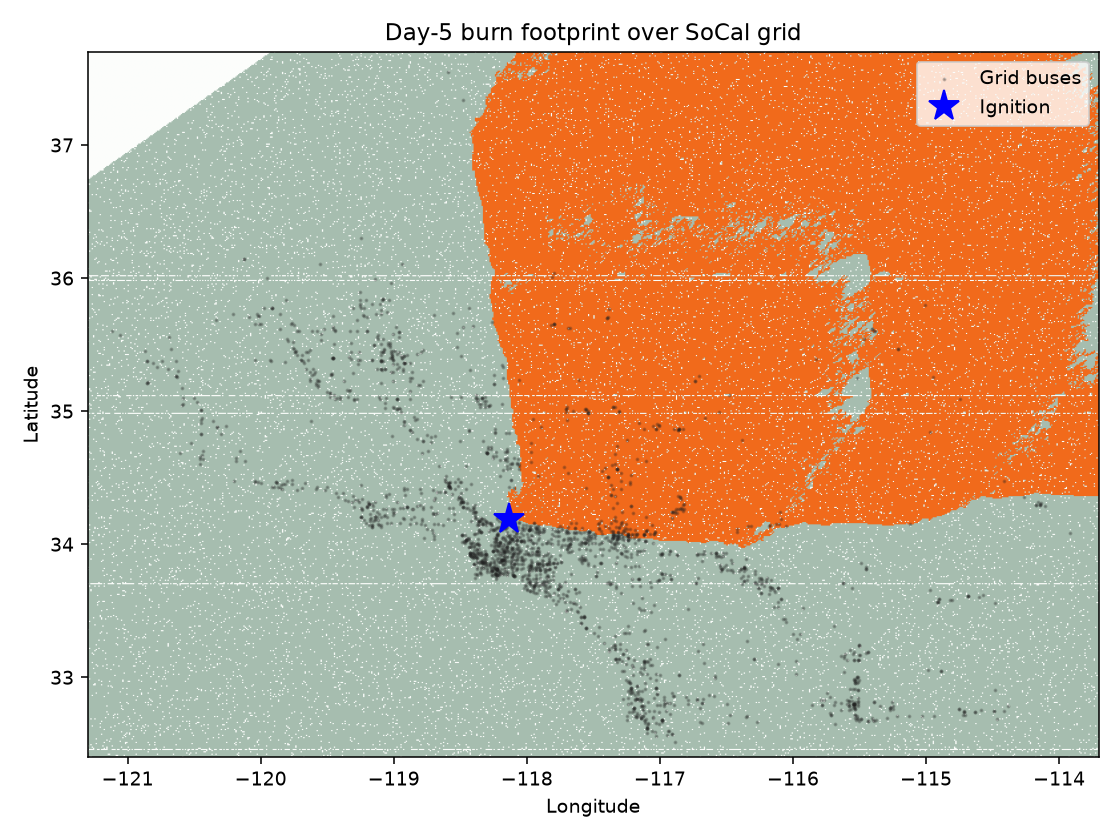
\includegraphics[width=\linewidth]{fire_perimeter_day5.png}\\[2pt]
      {\scriptsize\color{csladarkgray}Simulated fire perimeter, day 5
       (\texttt{analysis/fire\_perimeter\_day5.png})}
    \end{column}
  \end{columns}
\end{frame}

\begin{frame}{The Research Gap}{Fire models and grid models rarely talk to each other}
  \begin{columns}[T,onlytextwidth]
    \begin{column}{0.31\textwidth}
      \begin{block}{Fire-centric}
        \small
        Detailed spread physics (Rothermel, Cell2Fire, FARSITE).\\[4pt]
        Infrastructure is \emph{absent} or a static value layer.
      \end{block}
    \end{column}
    \begin{column}{0.31\textwidth}
      \begin{block}{Grid-centric}
        \small
        Detailed power-flow and contingency analysis.\\[4pt]
        Fire enters as an \emph{exogenous} outage list or PSPS scenario.
      \end{block}
    \end{column}
    \begin{column}{0.34\textwidth}
      \begin{alertblock}{This testbed}
        \small
        Validated CA spread \emph{and} full power-flow re-solve, every step,
        on \gold{one shared geospatial frame}.\\[4pt]
        A burned cell and its electrical asset are always co-registered.
      \end{alertblock}
    \end{column}
  \end{columns}
  \vskip6pt
  \begin{itemize}
    \item Mao et al. (2026) explicitly call for \emph{feedback-coupled
          fire/grid simulations}.
    \item Without coupling you cannot ask: \emph{did that suppression tactic
          protect the right cells?}
  \end{itemize}
  \srcnote{Source: Veith \& Sultan, ``When Wildfire Breaks the Grid'', Sec.~1--2.}
\end{frame}

\begin{frame}{GUARDIAN and the Curse of Rarity}{The wider research programme}
  \begin{columns}[T,onlytextwidth]
    \begin{column}{0.52\textwidth}
      \textbf{The problem}
      \begin{itemize}
        \item DRL controllers are trained on data they have seen.
        \item Catastrophic events are, by definition, \gold{rare} --- they sit
              outside the training distribution.
        \item So agents fail \emph{exactly} when resilience matters most.
              This is the \gold{Curse of Rarity}.
      \end{itemize}
      \vskip6pt
      \textbf{The GUARDIAN answer}
      \begin{itemize}
        \item Synthesise physically plausible worst-case worlds from
              curated GIS data.
        \item Train foundation policies against them via
              \gold{Adversarial Resilience Learning (ARL)}.
      \end{itemize}
    \end{column}
    \begin{column}{0.46\textwidth}
      \begin{block}{Project facts}
        \small
        NATO Science for Peace and Security Multi-Year Project.\\[3pt]
        Pillars: energy security, environmental hazards, advanced AI.\\[3pt]
        Dual PI: \textbf{Veith} (OFFIS, DE) \& \textbf{Sultan}
        (Cal State LA, US).\\[3pt]
        Validation cases: SoCal wildfire cascades; Central European
        severe-weather grid failures.
      \end{block}
      \vskip2pt
      {\scriptsize\color{csladarkgray}Motivating precedent: the Feb.\ 2022
       KA-SAT cyberattack disabled 5{,}800 wind turbines
       ($\approx$11\,GW) across Central Europe.}
    \end{column}
  \end{columns}
\end{frame}

\begin{frame}{GUARDIAN System Architecture}{Where this repository sits in the bigger picture}
  \centering
  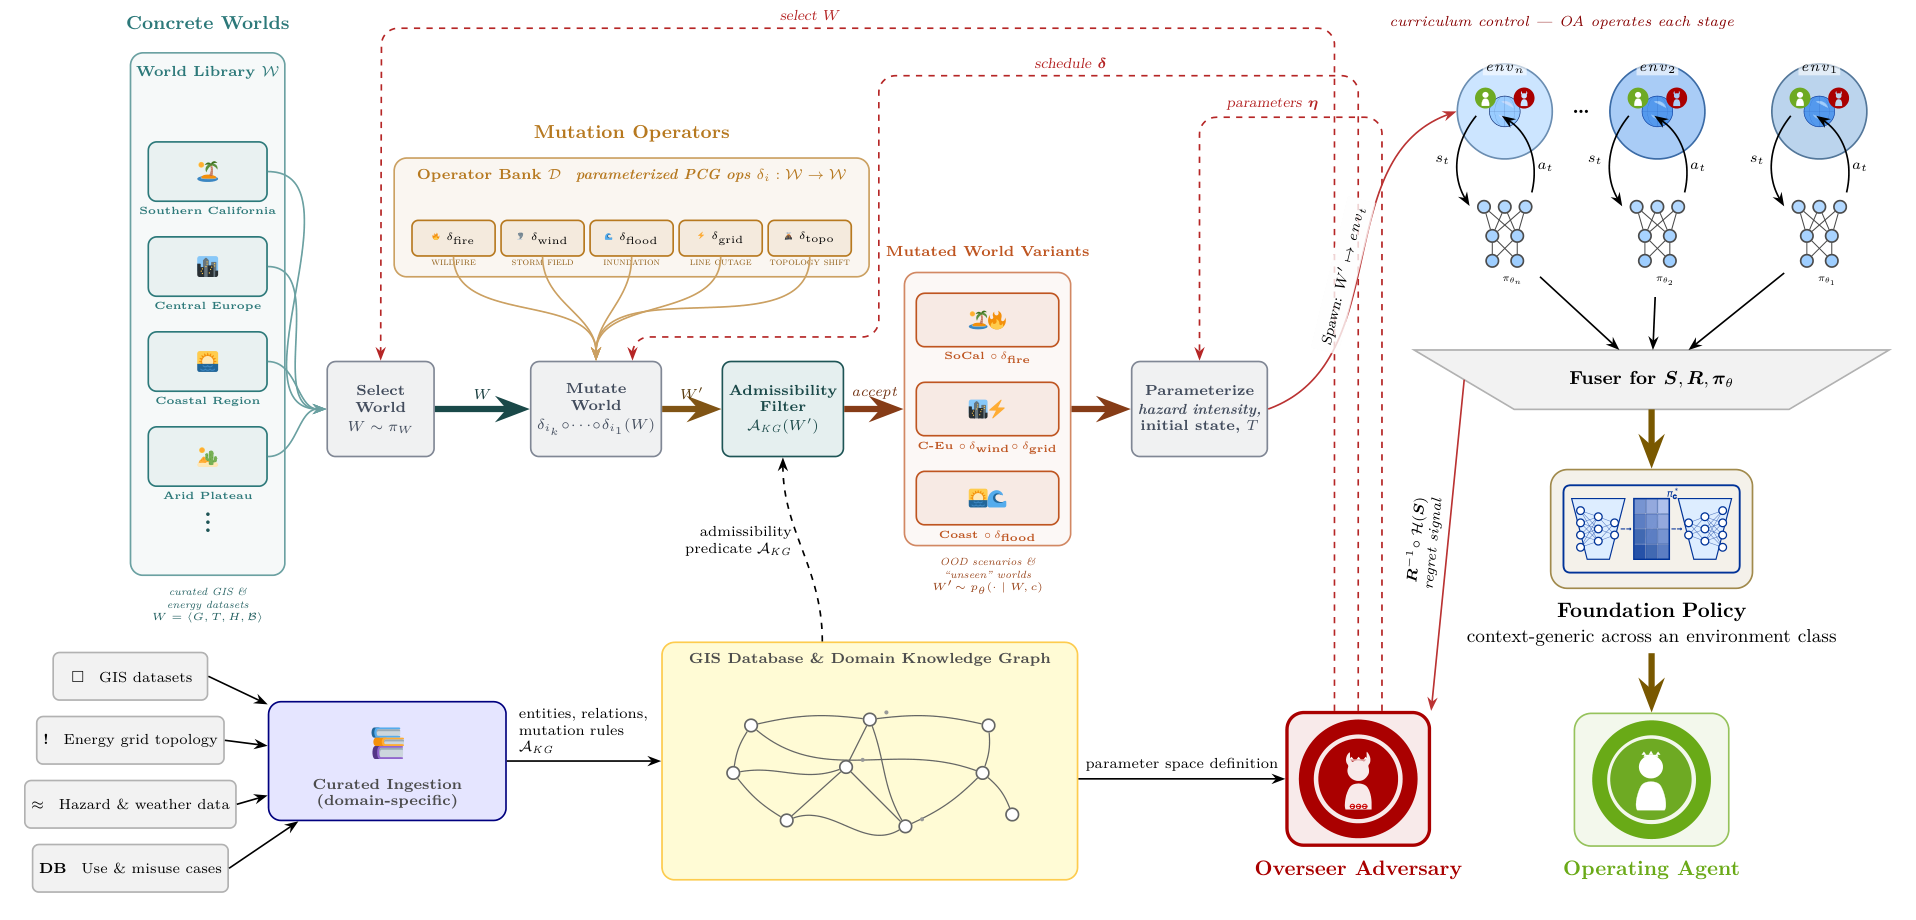
\includegraphics[width=0.88\textwidth]{guardian_architecture.png}
  \vskip2pt
  {\scriptsize\color{csladarkgray}%
   \textbf{This repository} implements the \emph{SoCal $\circ$ $\delta_{\text{fire}}$}
   branch: one concrete world, one mutation operator, one operating agent.}
  \srcnote{Figure 2 from Sultan, Logemann \& Veith, ``GUARDIAN''.}
\end{frame}

\begin{frame}{What You Will Take Away}{Learning objectives}
  \begin{enumerate}
    \item \textbf{Purpose} --- what question this testbed is built to answer,
          and what it deliberately does \emph{not} model.
    \item \textbf{Concepts} --- the constrained-mutation formalism
          $\mathrm{CMA}=(S,\tau,D,\Theta)$ and where learning enters.
    \item \textbf{Architecture} --- how the geospatial, fire, grid and
          agent layers fit together in palaestrAI.
    \item \textbf{Navigation} --- which directory and which module to open
          for a given question.
    \item \textbf{Operation} --- the exact commands to reproduce every
          published figure.
    \item \textbf{Research} --- open ARL questions that are available as
          thesis topics.
  \end{enumerate}
  \vskip6pt
  \begin{block}{Prerequisite}
    \small Basic palaestrAI familiarity. Slide~8 is a short refresher; a
    one-page reminder of experiment runs, environments and muscles.
  \end{block}
\end{frame}

% =====================================================================
\section{Purpose and Conceptual Model}
% =====================================================================

\begin{frame}{What the Repository Delivers}{Four deliverables}
  \begin{columns}[T,onlytextwidth]
    \begin{column}{0.48\textwidth}
      \begin{block}{1 --- NOAA-enriched MIDAS scenario}
        \small SoCal co-simulation scenario with weather switched from
        DWD Bremen to \gold{NOAA HRRR} reanalysis, inside the scenario.
      \end{block}
      \begin{block}{2 --- palaestrAI environment}
        \small SoCal MIDAS wrapped as a first-class
        \code{palaestrai.environment.Environment}, plus an experiment run
        file.
      \end{block}
    \end{column}
    \begin{column}{0.48\textwidth}
      \begin{block}{3 --- Wildfire agent (GUARDIAN CMA)}
        \small Cellular automaton driven by the Overseer-Adversary
        parameter vector $\Theta$, over the full SoCal GIS footprint;
        optional PostGIS layer.
      \end{block}
      \begin{block}{4 --- Five-day co-simulation}
        \small 120\,h Santa-Ana wildfire/grid run with KPIs, plots and a
        generated report.
      \end{block}
    \end{column}
  \end{columns}
  \srcnote{Source: repository \texttt{README.md}.}
\end{frame}

\begin{frame}{palaestrAI Refresher}{The five nouns you need for this deck}
  \begin{columns}[T,onlytextwidth]
    \begin{column}{0.5\textwidth}
      \small
      \begin{description}
        \item[Experiment run] A declarative YAML document: environments,
              agents, phases, termination conditions. Fully reproducible ---
              the document \emph{is} the experiment.
        \item[Environment] Owns state, publishes \gold{sensors}, accepts
              \gold{actuators}, is stepped by a simulation controller.
        \item[Agent] A \gold{Brain} (learns, lives in the Learner process)
              plus one or more \gold{Muscles} (act, live in RolloutWorkers).
      \end{description}
    \end{column}
    \begin{column}{0.48\textwidth}
      \small
      \begin{description}
        \item[Objective] Maps sensor readings to scalar reward. Separate
              from the environment, so several agents can score the same
              world differently.
        \item[Store] Every sensor, actuator and reward is written to a
              database, so analysis scripts read results instead of
              re-running simulations.
      \end{description}
      \vskip6pt
      \begin{alertblock}{Two conventions used throughout}
        \small
        \code{TakingTurnsSimulationController} --- agents act in a fixed
        order, not simultaneously.\\[3pt]
        \code{DummyBrain} --- an agent that \emph{acts but never learns}.
      \end{alertblock}
    \end{column}
  \end{columns}
\end{frame}

\begin{frame}{End-to-End Simulation Loop}{One timestep}
  \centering
  \begin{tikzpicture}[
      node distance=6mm and 5mm,
      box/.style={draw=cslablack, line width=0.8pt, fill=cslatintgray,
                  rounded corners=2pt, align=center, inner sep=4pt,
                  text width=19mm, font=\tiny},
      gbox/.style={box, fill=cslagold!35},
      ar/.style={-{Latex[length=1.8mm]}, line width=0.9pt, draw=csladarkgray}]

    \node[gbox] (fire) {\textbf{Wildfire CA}\\$\tau$ advances\\burn state $S$};
    \node[box, right=of fire] (ff) {\textbf{Firefighter}\\suppression\\mutations};
    \node[box, right=of ff]   (dm) {\textbf{Damage mapper}\\$D$: cells\\$\rightarrow$ assets};
    \node[box, right=of dm]   (pf) {\textbf{Power flow}\\pandapower\\re-solve};
    \node[gbox, right=of pf]  (mt) {\textbf{Metrics}\\SAIDI, served\\MW, voltage};

    \draw[ar] (fire) -- (ff);
    \draw[ar] (ff) -- (dm);
    \draw[ar] (dm) -- (pf);
    \draw[ar] (pf) -- (mt);

    \node[draw=cslaeaglegold, line width=0.8pt, dashed, rounded corners=3pt,
          fit=(fire)(mt), inner sep=8pt] (frame) {};
    \node[below=1pt of frame, font=\scriptsize\itshape, text=cslaeaglegold]
      {all four stages share one geospatial reference frame};
  \end{tikzpicture}
  \vskip8pt
  \begin{itemize}
    \item Agents act in \gold{fixed turn order}:
          \code{wildfire} $\rightarrow$ \code{firefighter} $\rightarrow$
          \code{damage\_mapper}.
    \item Conflicting cell edits are resolved by \emph{priority}, not by turn
          order --- so the result is deterministic.
  \end{itemize}
\end{frame}

\begin{frame}{Mental Model: $\mathrm{CMA} = (S, \tau, D, \Theta)$}{The GUARDIAN constrained-mutation automaton}
  \begin{columns}[T,onlytextwidth]
    \begin{column}{0.5\textwidth}
      \begin{block}{$S$ --- state}
        \small \code{int8} cell grid, co-registered with the raster.
        \code{UNBURNED}\,0, \code{BURNING}\,1, \code{BURNED\_OUT}\,2,
        \code{SUPPRESSED}\,3, \code{CONTAINED}\,5.
      \end{block}
      \begin{block}{$\tau$ --- transition}
        \small The CA sub-step (\code{dt\_cma\_min}, default 5\,min). Each
        burning cell attempts to ignite its 8 Moore neighbours.
      \end{block}
    \end{column}
    \begin{column}{0.5\textwidth}
      \begin{block}{$D$ --- damage map}
        \small Fails buses whose cell is burning or burned, and overhead
        lines inside a radiant-heat clearance buffer.
      \end{block}
      \begin{alertblock}{$\Theta$ --- the adversary's handle}
        \small Ignition point(s), wind vector, dead-fuel moisture, and the
        global ROS multiplier $\kappa$ ($1 \le \kappa \le 8$).\\[3pt]
        \textbf{$\Theta$ is the entire attack surface} --- everything else
        is physics.
      \end{alertblock}
    \end{column}
  \end{columns}
  \srcnote{Source: \texttt{docs/CMA\_AGENT.md}, \texttt{wildfire\_cma/cma.py}.}
\end{frame}

\begin{frame}{What Is --- and Is Not --- Learning}{The single most common misreading of this repo}
  \centering
  \small
  \begin{tabular}{@{}l l l@{}}
    \toprule
    \textbf{Component} & \textbf{Brain} & \textbf{Learns?}\\
    \midrule
    Wildfire (GUARDIAN CMA) & \code{DummyBrain} & \textbf{No} --- constrained
      mutation operator driven by $\Theta$\\
    Damage mapper           & \code{DummyBrain} & \textbf{No} --- deterministic
      consequence model\\
    Firefighter v0.3--v0.5  & scripted doctrine & \textbf{No} --- expert
      incident-command heuristics\\
    Firefighter v0.7        & \code{FirefighterSacBrain} & \textbf{Yes} ---
      SAC with CQL, bootstrapped offline\\
    \bottomrule
  \end{tabular}
  \vskip10pt
  \begin{columns}[T,onlytextwidth]
    \begin{column}{0.49\textwidth}
      \begin{block}{Why the fire does not learn}
        \small This is a deliberate, paper-faithful choice. The published
        work positions the CA as \emph{the calibrated, validated substrate}
        on which a learned scenario-generation loop can \emph{later} be
        built.
      \end{block}
    \end{column}
    \begin{column}{0.49\textwidth}
      \begin{alertblock}{Why that matters to you}
        \small Turning $\Theta$ from a calibrated constant into a learned
        adversarial policy is the open door into ARL --- and the subject of
        Sec.~6 of this talk.
      \end{alertblock}
    \end{column}
  \end{columns}
\end{frame}

% =====================================================================
\section{Technical Architecture}
% =====================================================================

\begin{frame}{Repository Map}{Where to look for what}
  \small
  \begin{tabular}{@{}>{\ttfamily}l p{0.63\textwidth}@{}}
    \toprule
    \textrm{\textbf{Directory}} & \textbf{Contents} \\
    \midrule
    wildfire\_cma/     & The CA itself: \code{cma.py} ($S$, $\tau$, $\Theta$),
                         \code{gis.py}, \code{damage.py},
                         \code{wind\_field.py}, \code{postgis.py}. Pure
                         \code{numpy}, no palaestrAI import. \\
    palaestrai\_socal/ & Environments (\code{gis\_world\_env.py},
                         \code{midas\_grid\_env.py}), all agents under
                         \code{agents/}, and every
                         \code{experiment*.yml}. \\
    socal\_grid/       & Geo-referenced pandapower model plus
                         \code{dispatch\_and\_run.py} (the convergence
                         recipe) and \code{build\_network.py}. \\
    midas\_socal/      & MIDAS scenario \code{socal\_midas.yml}, NOAA
                         weather provider, \code{prepare\_midas.py},
                         \code{run\_sim.sh}. \\
    analysis/          & Drivers, report generators, timelapse builders and
                         the committed result figures. \\
    data/              & GIS layers, DEM fetcher, CAL FIRE perimeters,
                         offline teacher datasets, CAISO load. \\
    docs/, tests/      & Design docs; $\approx$30 test modules
                         (\textbf{235 passing} as of v0.7). \\
    \bottomrule
  \end{tabular}
  \vskip5pt
  {\scriptsize\color{csladarkgray}Start reading at
   \texttt{wildfire\_cma/cma.py} --- it has no framework dependencies.}
\end{frame}

\begin{frame}{Geospatial Layer}{The shared reference frame}
  \begin{columns}[T,onlytextwidth]
    \begin{column}{0.55\textwidth}
      \begin{itemize}
        \item Footprint \code{SOCAL\_BOUNDS} $=(-121.3,\,32.4,\,-113.7,\,37.7)$,
              EPSG:4326. Row 0 is the \emph{north} edge.
        \item Three raster sources, in order of fidelity:
          \begin{itemize}
            \item \code{from\_rasters()} --- real LANDFIRE FBFM40 fuel +
                  3DEP elevation (needs \code{rasterio}).
            \item \code{socal\_from\_srtm()} --- SRTM GL3 ($\approx$90\,m)
                  via OpenTopography, 4$\times$3 tile mosaic, resampled to
                  a $600\times760$ model grid.
            \item \code{synthetic\_socal()} --- deterministic fallback used
                  by CI.
          \end{itemize}
        \item Degrades \emph{gracefully}: a missing DEM cache silently
              falls back to synthetic terrain.
      \end{itemize}
      \begin{alertblock}{Scale trap}
        \small On the statewide grid one cell $\approx$\,947\,m. Retardant
        drops are sub-cell there --- which is why fine grids
        ($\approx$50\,m) are used for suppression studies.
      \end{alertblock}
    \end{column}
    \begin{column}{0.43\textwidth}
      \centering
      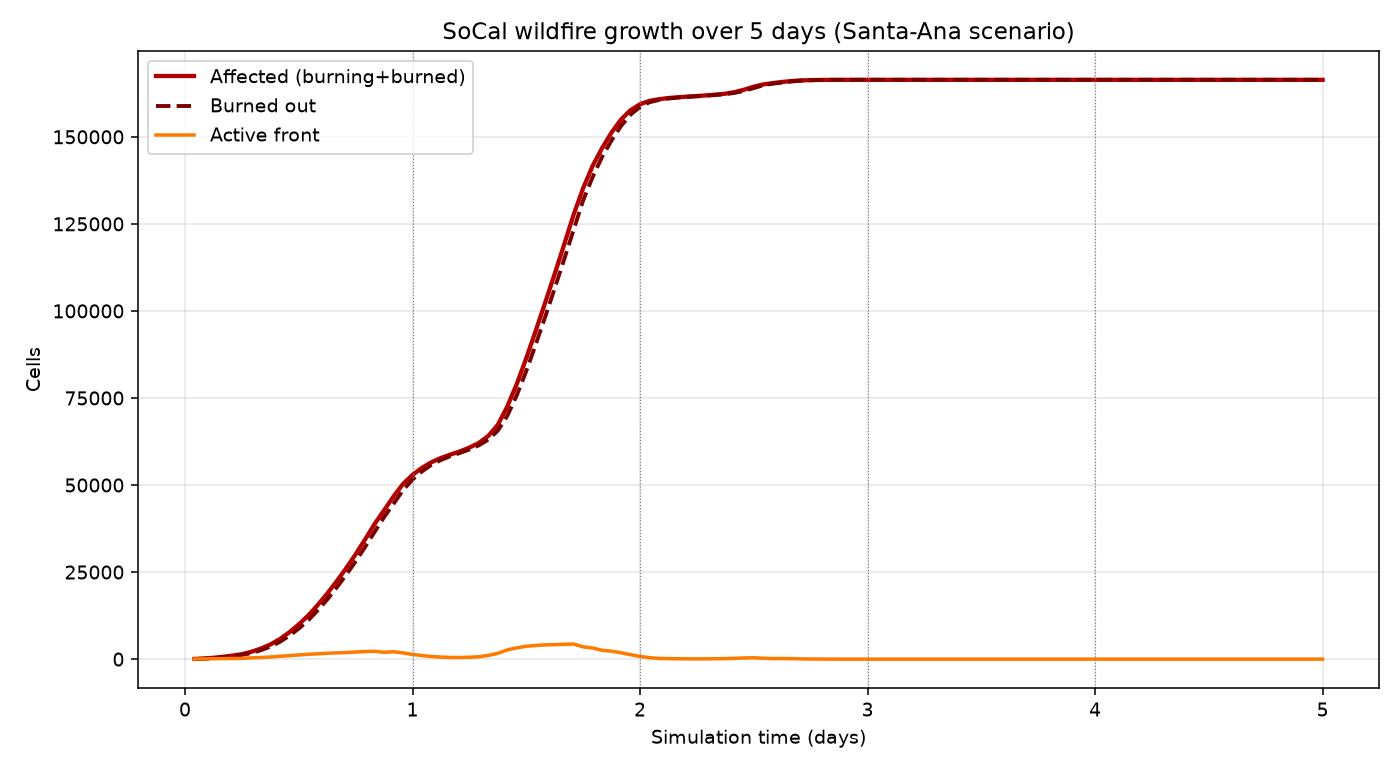
\includegraphics[width=\linewidth]{fire_growth.png}\\[2pt]
      {\scriptsize\color{csladarkgray}Fire growth on the statewide raster
       (\texttt{analysis/fire\_growth.png})}
    \end{column}
  \end{columns}
\end{frame}

\begin{frame}{Wildfire Spread Kernel}{Rothermel-derived, wind- and slope-modulated}
  \begin{columns}[T,onlytextwidth]
    \begin{column}{0.56\textwidth}
      \textbf{Rate of spread}
      \[
        R(i,j \to i',j') \;=\; \kappa \cdot R^{0}(i,j)
          \cdot \varphi_w(u,\theta) \cdot \varphi_s(z,\theta)
      \]
      \textbf{Ignition probability per sub-step}
      \[
        p \;=\; 1 - \exp\!\left(-\,R \cdot \Delta t_{\mathrm{CMA}} / \delta\right)
      \]
      \small
      \begin{itemize}
        \item $R^{0}$ --- base ROS by fuel class, damped by dead-fuel
              moisture through the Rothermel coefficient $\eta_m$; zero
              above \code{FUEL\_MX\_EXTINCTION}.
        \item $\varphi_w = \exp(c\,u\cos\alpha)$, $c=0.25$, tuned so
              $\approx$20\,m/s Santa-Ana wind reproduces the observed
              \gold{60--80\,m/min} fronts.
        \item $\varphi_s = 1 + 5.275\tan^{2}(\text{slope})\cdot$ upslope
              alignment.
        \item $\delta$ = cell size in m ($\times\sqrt{2}$ diagonally).
              A neighbour ignites iff \code{rng.random() < p} --- the only
              stochastic element, and it is seeded.
      \end{itemize}
    \end{column}
    \begin{column}{0.42\textwidth}
      \centering\small
      \begin{tabular}{@{}c l r@{}}
        \toprule
        \textbf{\#} & \textbf{Fuel class} & \textbf{$R^{0}$}\\
                    &                     & {\scriptsize m/min}\\
        \midrule
        0 & non-burnable        & 0.0\\
        1 & grass (GR)          & 4.0\\
        2 & grass-shrub (GS)    & 2.5\\
        3 & shrub / chaparral (SH) & \textbf{3.2}\\
        4 & timber-understory (TU) & 1.2\\
        5 & timber-litter (TL)  & 0.8\\
        6 & slash-blowdown (SB) & 1.5\\
        \bottomrule
      \end{tabular}
      \vskip4pt
      {\scriptsize\color{csladarkgray}Class 3 dominates SoCal.
       \texttt{gis.fbfm40\_to\_class()} maps the 40 Scott-Burgan models
       onto these seven.}
    \end{column}
  \end{columns}
\end{frame}

\begin{frame}{Power Grid Model}{The electrical side}
  \begin{columns}[T,onlytextwidth]
    \begin{column}{0.55\textwidth}
      \begin{itemize}
        \item \gold{2{,}294 buses / 2{,}595 lines}, geo-referenced
              pandapower model (\code{socal\_grid/socal\_grid.json},
              EPSG:4326, $\approx$5.9\,MB).
        \item Built from open data: OSM substations, transmission lines,
              power plants, city populations, CAISO load profiles.
        \item An \emph{illustrative} distribution topology --- deliberately
              \textbf{not} a utility feeder model.
        \item Customers derived via \code{CUSTOMERS\_PER\_MW = 200.0}.
      \end{itemize}
      \begin{alertblock}{Convergence gotcha --- read this first}
        \small Raw \code{pp.runpp()} on \code{socal\_grid.json}
        \textbf{diverges}. Always go through
        \code{socal\_grid/dispatch\_and\_run.py} --- ``config D'':
        strengthen the network, co-locate dispatch, then solve with
        \gold{Iwamoto Newton-Raphson}.
      \end{alertblock}
    \end{column}
    \begin{column}{0.43\textwidth}
      \centering
      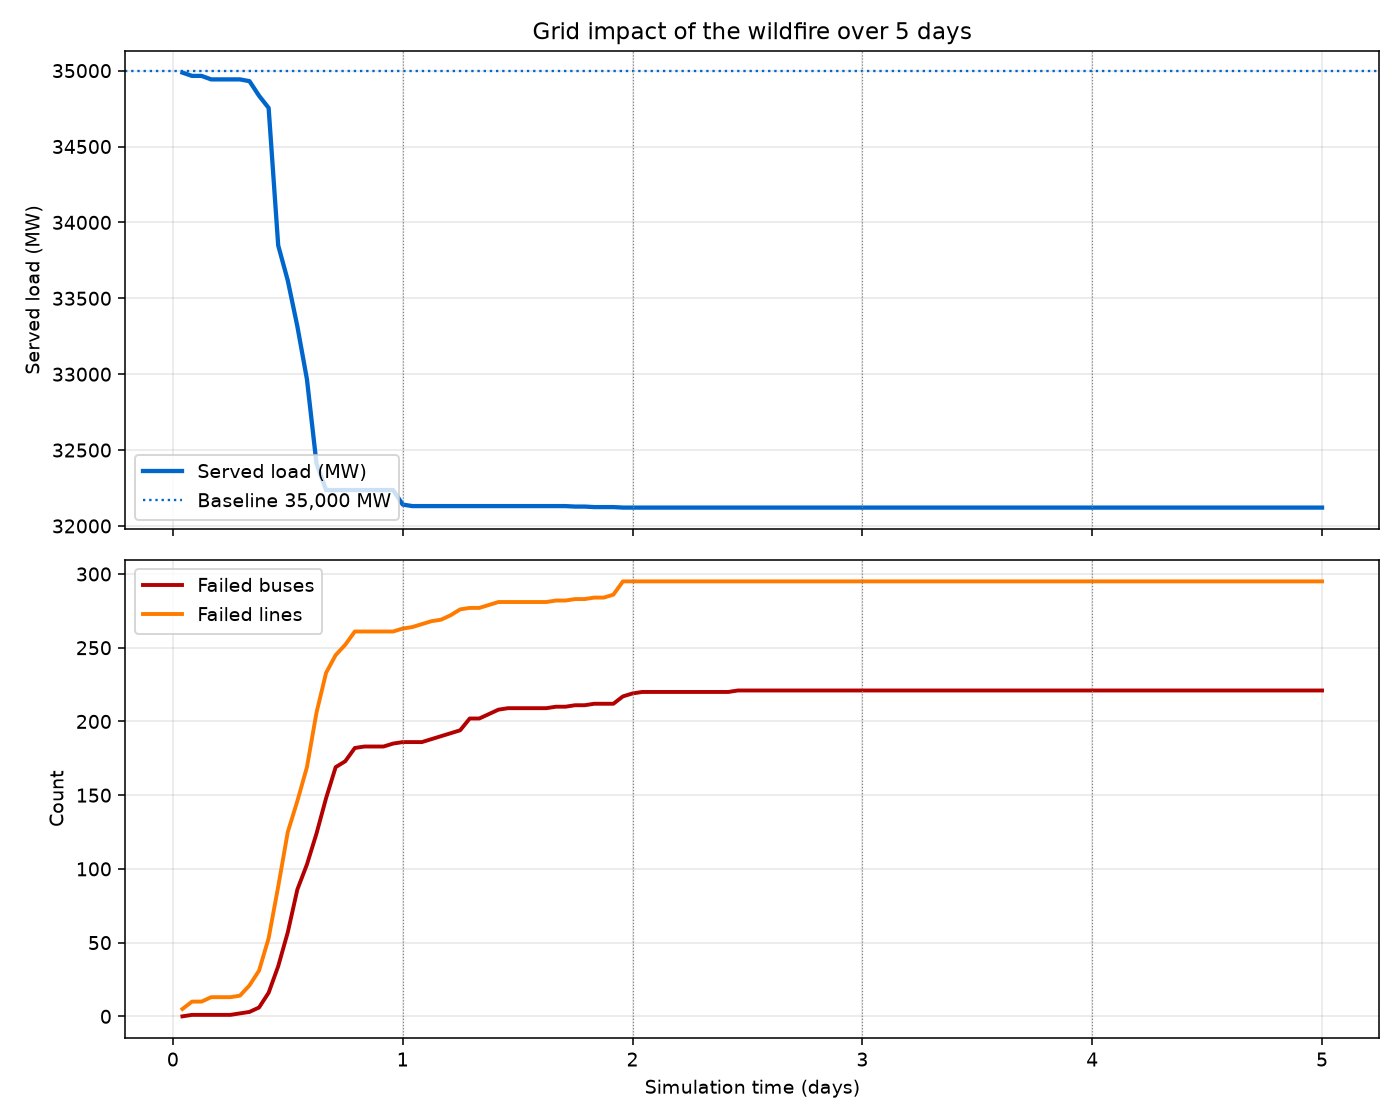
\includegraphics[width=\linewidth]{grid_impact.png}\\[2pt]
      {\scriptsize\color{csladarkgray}Grid impact over the five-day run
       (\texttt{analysis/grid\_impact.png})}
    \end{column}
  \end{columns}
\end{frame}

\begin{frame}{Damage Mapping}{From burned cells to de-energised assets}
  \begin{columns}[T,onlytextwidth]
    \begin{column}{0.52\textwidth}
      \textbf{The mechanism}
      \begin{enumerate}
        \small
        \item Every bus and every line endpoint is projected onto the
              raster once, at setup.
        \item A bus whose cell is \code{BURNING} or \code{BURNED\_OUT}
              is de-energised.
        \item An overhead line is removed if its corridor intersects a
              burning cell within the \emph{radiant-heat clearance
              buffer}.
        \item Power flow is re-solved; SAIDI and served MW are recorded.
      \end{enumerate}
      \vskip4pt
      \begin{block}{Implementation note}
        \small mosaik exposes no \code{in\_service} actuator for buses or
        lines. So under MIDAS the damage is applied as a
        \gold{load-shed trip}: write
        \code{...load-<bus>-<idx>.p\_mw} $\rightarrow 0$.
      \end{block}
    \end{column}
    \begin{column}{0.46\textwidth}
      \begin{alertblock}{Mutation arbitration}
        \small Several agents may edit the same cell in one step. A fixed
        priority makes the outcome independent of turn order:
        \vskip3pt
        \centering
        \code{BURNED\_OUT} (terminal) $>$ \code{SUPPRESSED} $>$
        \code{FLOODED} $>$ \code{BURNING} $>$ \code{UNBURNED}
        \vskip3pt
        \raggedright
        See \code{spaces.arbitrate\_mutations}. Suppression is not
        permanent: the environment reverts a cell after
        \code{SUPPRESS\_PERSIST\_STEPS}\,$=12$.
      \end{alertblock}
    \end{column}
  \end{columns}
  \srcnote{Source: \texttt{docs/CMA\_AGENT.md}, \texttt{docs/AGENTS.md}.}
\end{frame}

\begin{frame}{Multi-Agent Architecture}{The v0.2 two-environment design}
  \centering
  \begin{tikzpicture}[
      font=\scriptsize,
      env/.style={draw=cslablack, line width=1pt, fill=cslagold!25,
                  rounded corners=3pt, align=center, inner sep=5pt,
                  text width=38mm},
      ag/.style={draw=csladarkgray, line width=0.8pt, fill=cslatintgray,
                 rounded corners=2pt, align=center, inner sep=4pt,
                 text width=26mm},
      ar/.style={-{Latex[length=1.8mm]}, line width=0.8pt, draw=csladarkgray},
      arg/.style={-{Latex[length=1.8mm]}, line width=0.9pt, draw=cslaeaglegold}]

    \node[env] (gis) at (0,0)
      {\textbf{\texttt{gis\_world}}\\\texttt{GisWorldEnvironment}\\
       {\tiny passive spatial substrate; owns hazard grid $S$ + static raster}};
    \node[env] (grid) at (7.4,0)
      {\textbf{\texttt{socal\_grid}}\\\texttt{SocalMidasGridEnvironment}\\
       {\tiny thin \texttt{MosaikEnvironment} subclass; stepped by mosaik}};

    \node[ag] (wf) at (-1.1,2.5) {\textbf{wildfire}\\{\tiny\texttt{WildfireCmaMuscle}}};
    \node[ag] (ff) at (1.9,2.5)  {\textbf{firefighter}\\{\tiny\texttt{FirefighterMuscle}}};
    \node[ag] (dm) at (5.6,2.5)  {\textbf{damage\_mapper}\\{\tiny\texttt{DamageMapperMuscle}}};

    \draw[ar] (gis.north west) ++(0.3,0) -- (wf.south);
    \draw[ar] (wf.south) ++(0.5,0) -- ++(0,-0.9);
    \draw[ar] (gis.north) -- (ff.south);
    \draw[ar] (gis.north east) ++(-0.3,0) -- (dm.south west);
    \draw[arg] (dm.south east) -- (grid.north west);

    \node[align=left, text width=32mm, font=\tiny, text=csladarkgray]
      at (-0.9,4.15)
      {reads \texttt{gis.*}\\writes \texttt{gis.cell\_mutations} (BURNING)};
    \node[align=left, text width=30mm, font=\tiny, text=csladarkgray]
      at (2.6,4.15)
      {writes SUPPRESSED /\\LAYER\_SUPPRESSION};
    \node[align=left, text width=34mm, font=\tiny, text=cslaeaglegold]
      at (7.0,3.6)
      {writes\\\texttt{...load-<bus>-<idx>.p\_mw} $\rightarrow 0$};

    \draw[arg, dashed] (gis.east) -- node[above, font=\tiny, text=cslaeaglegold]
      {shared frame} (grid.west);
  \end{tikzpicture}
  \vskip6pt
  \begin{itemize}
    \item \code{gis\_world} is \gold{hazard-agnostic}: it steps no dynamics,
          it only applies \code{gis.cell\_mutations} and re-publishes
          telemetry. Wildfire today, flood or storm tomorrow.
    \item Ignition is an \emph{agent parameter}
          (\code{ignition\_points}, \code{ignition\_step}), \textbf{not} an
          environment actuator.
  \end{itemize}
\end{frame}

\begin{frame}{Firefighting Model Evolution}{Five releases, increasing realism}
  \centering
  \begin{tikzpicture}[font=\scriptsize, node distance=0mm]
    \draw[line width=2.5pt, color=cslagold] (0,0) -- (11.6,0);
    \foreach \x/\v/\t/\d in {%
      0.4/v0.3/Aero-tankers/{one knob: \texttt{n\_planes}},
      3.0/v0.4/Incident command/{+helos, crews, dozers, engines, doctrine},
      5.7/v0.5/Calibration/{tuned to real CAL FIRE perimeters},
      8.2/v0.6/Timelapse rework/{Esri satellite basemap, no API key},
      10.6/v0.7/Learning agent/{SAC + CQL from an offline teacher}}
    {
      \fill[cslablack] (\x,0) circle (2.6pt);
      \node[above=6pt, align=center, text width=23mm] at (\x,0)
        {\textbf{\v}\\{\tiny\t}};
      \node[below=6pt, align=center, text width=25mm, text=csladarkgray] at (\x,0)
        {\tiny\d};
    }
  \end{tikzpicture}
  \vskip14pt
  \begin{columns}[T,onlytextwidth]
    \begin{column}{0.49\textwidth}
      \begin{block}{Tunable knobs (v0.4 onward)}
        \small \code{n\_planes}, \code{n\_helos}, \code{n\_crews},
        \code{n\_dozers}, \code{n\_engines},
        \code{doctrine} $\in$ \{\code{auto}, \code{direct},
        \code{indirect}\}, \code{protect\_assets}.
      \end{block}
    \end{column}
    \begin{column}{0.49\textwidth}
      \begin{alertblock}{Physical constraints are enforced}
        \small Fleets degrade above \code{DEGRADE\_WIND\_MS}\,$=13$\,m/s and
        are \gold{grounded} at \code{GROUND\_WIND\_MS}\,$=18$\,m/s --- so a
        25\,m/s high-wind Eaton run is genuinely unchanged by air support.
      \end{alertblock}
    \end{column}
  \end{columns}
  \srcnote{Source: \texttt{CHANGELOG.md}, \texttt{agents/firefighter\_core.py}.}
\end{frame}

% =====================================================================
\section{Existing Results}
% =====================================================================

\begin{frame}{Calibration Against Real Fires}{The credibility argument}
  \begin{columns}[T,onlytextwidth]
    \begin{column}{0.46\textwidth}
      \centering
      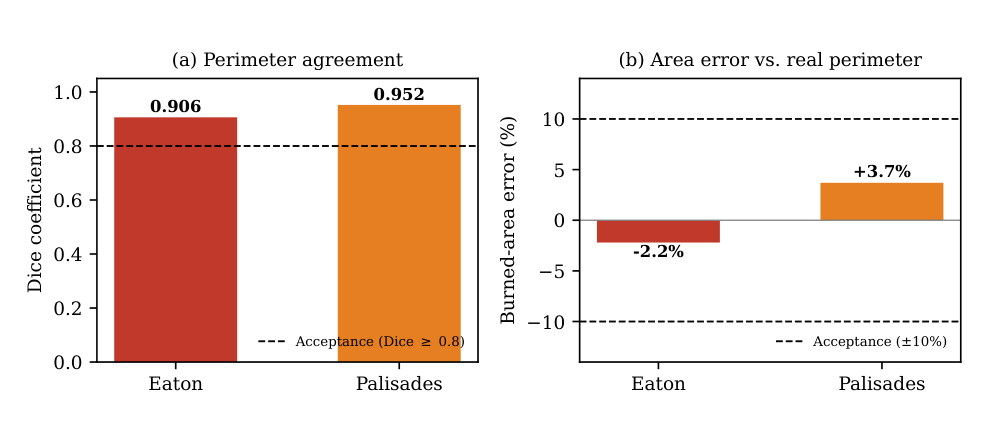
\includegraphics[width=\linewidth]{esm_fig1_calibration.png}\\[3pt]
      {\scriptsize\color{csladarkgray}Figure 1 from ``When Wildfire Breaks
       the Grid''.}
    \end{column}
    \begin{column}{0.52\textwidth}
      \small
      \begin{tabular}{@{}l r r c@{}}
        \toprule
        \textbf{Fire} & \textbf{Dice} & \textbf{Area err.} & \textbf{Verdict}\\
        \midrule
        Eaton     & 0.906 & $-2.2\,\%$ & PASS\\
        Palisades & 0.952 & $+3.7\,\%$ & PASS\\
        \bottomrule
      \end{tabular}
      \vskip6pt
      \begin{itemize}
        \item Acceptance bar: Dice $\ge 0.8$ \textbf{and}
              $|\text{area}\,\%| \le 10$. Both fires clear it.
        \item Reference: official CAL FIRE perimeters at env step 60.
              Eaton 13{,}786 vs 14{,}102\,ac; Palisades 24{,}677 vs
              23{,}799\,ac.
      \end{itemize}
      \begin{alertblock}{Honest caveat}
        \small Without containment the free-running CA \emph{overshoots} by
        $+145\,\%$ (Eaton) and $+129\,\%$ (Palisades). The match relies on
        \code{wind\_field.py}: perimeter-informed wind, fuel reclassification
        and \code{contain\_burnable\_footprint(..., margin\_cells=2)}.
      \end{alertblock}
    \end{column}
  \end{columns}
\end{frame}

\begin{frame}{Five-Day Santa-Ana Baseline}{The headline scenario}
  \begin{columns}[T,onlytextwidth]
    \begin{column}{0.5\textwidth}
      \centering
      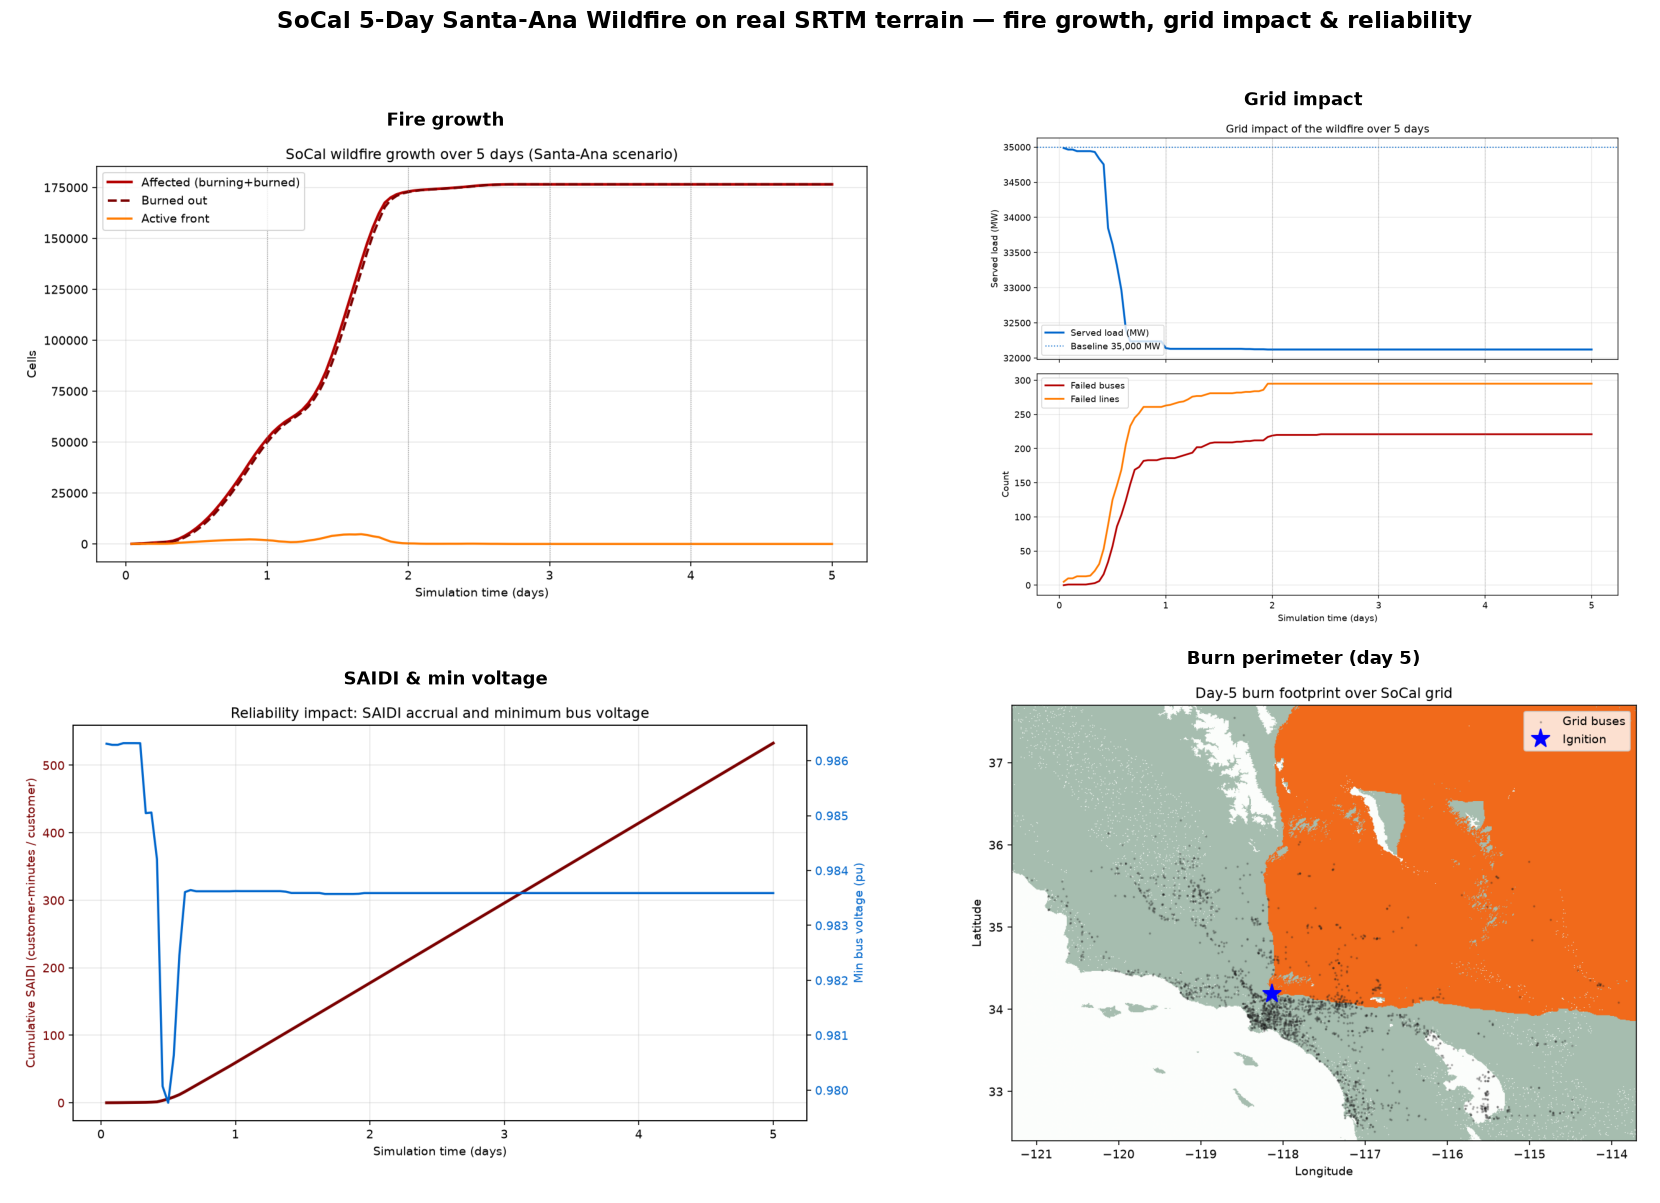
\includegraphics[width=\linewidth]{five_day_combined.png}\\[2pt]
      {\scriptsize\color{csladarkgray}\texttt{analysis/five\_day\_combined.png}}
    \end{column}
    \begin{column}{0.48\textwidth}
      \small
      \textbf{Setup} --- 120 hourly steps, seed 47, synthetic
      $600\times760$ raster. Strong dry offshore wind on days 1--3,
      marine-layer recovery on days 4--5.
      \vskip5pt
      \textbf{Outcome}
      \begin{itemize}
        \item Served load $\approx$35{,}000\,MW $\rightarrow$
              \gold{31{,}328\,MW}
        \item $\approx$213 buses and $\approx$327 lines de-energised
        \item Peak $\approx$\gold{734{,}000 customers} disconnected, around
              day 2.5
        \item Final burn footprint $\approx$166{,}000 cells
        \item Power flow converged \gold{120/120} steps
      \end{itemize}
      \vskip3pt
      {\scriptsize\color{csladarkgray}Reproduce with
       \texttt{python analysis/run\_5day.py --max-steps 120}.}
    \end{column}
  \end{columns}
\end{frame}

\begin{frame}{Suppression Counterfactuals}{Four phases of incident response}
  \begin{columns}[T,onlytextwidth]
    \begin{column}{0.52\textwidth}
      \centering
      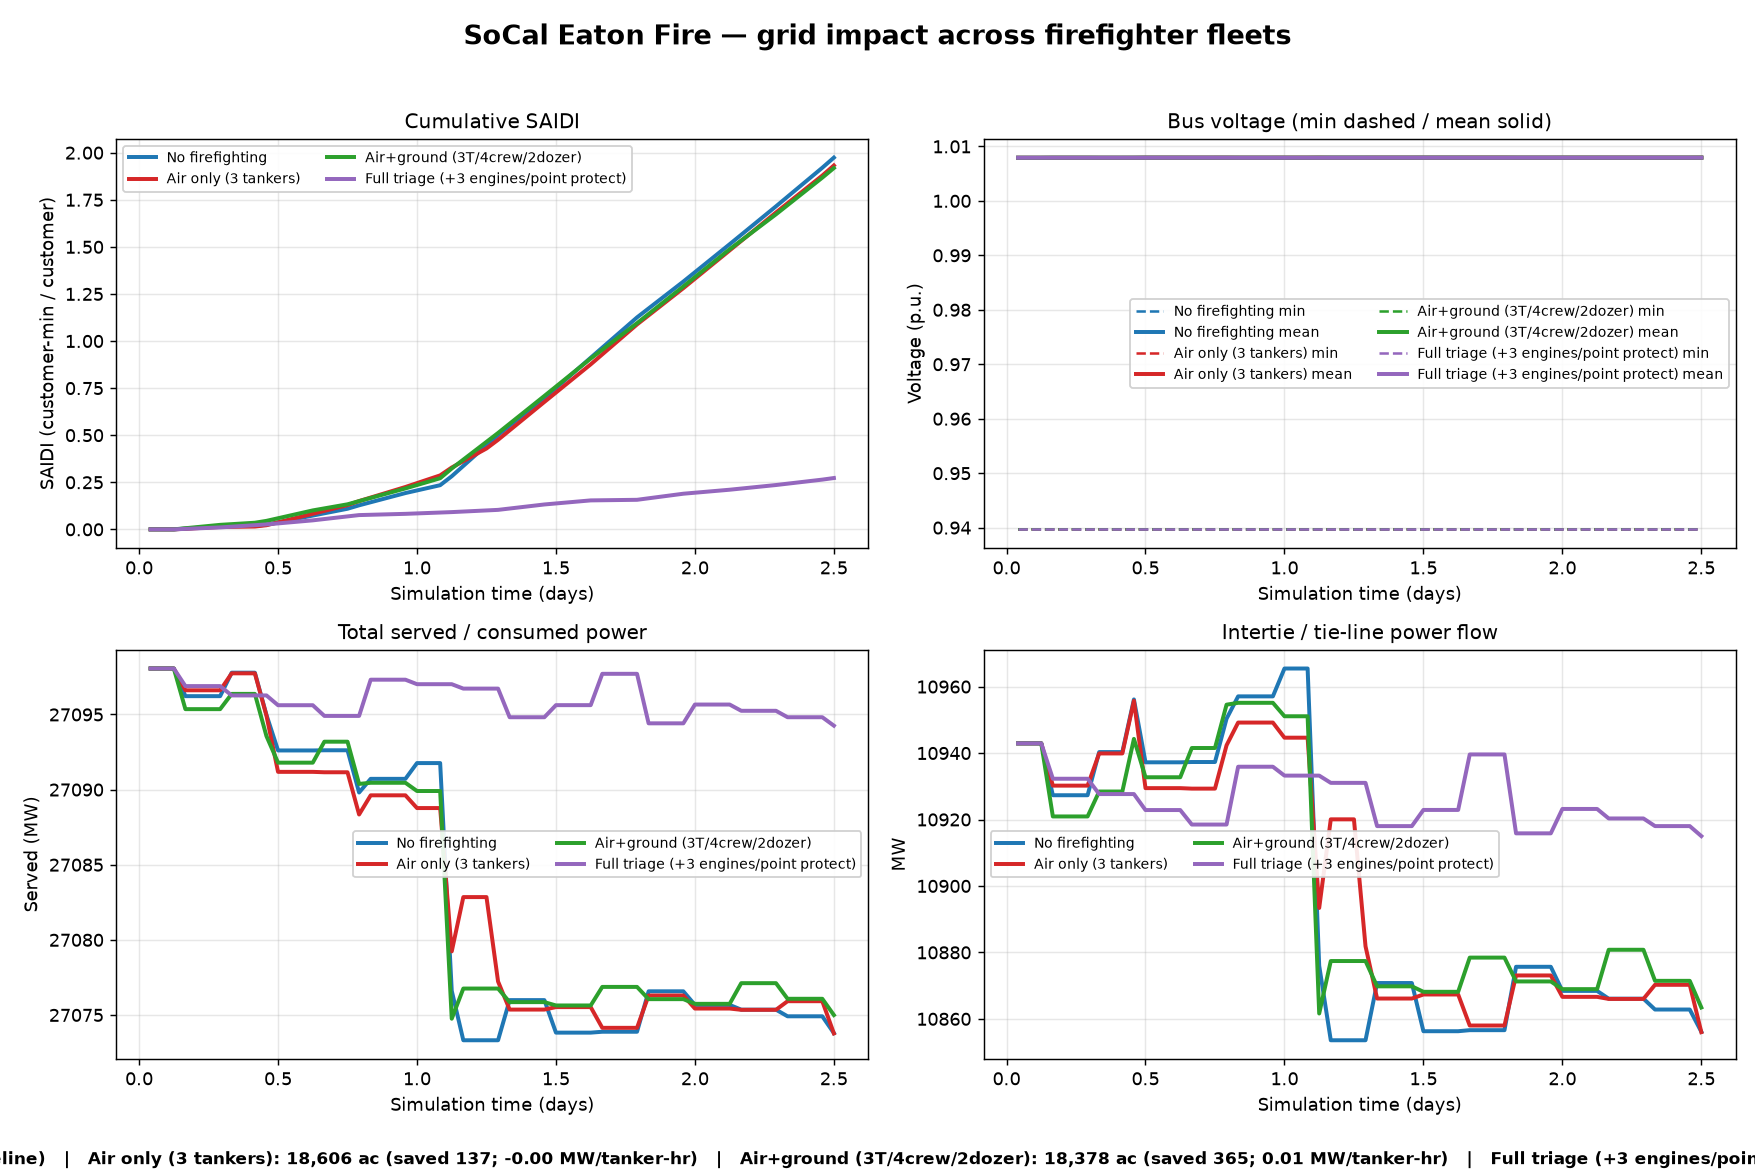
\includegraphics[width=\linewidth]{grid_metrics_v04.png}\\[2pt]
      {\scriptsize\color{csladarkgray}\texttt{analysis/grid\_metrics\_v04.png}}
    \end{column}
    \begin{column}{0.46\textwidth}
      \small
      \begin{tabular}{@{}l r r@{}}
        \toprule
        \textbf{Phase} & \textbf{Acres saved} & \textbf{SAIDI}\\
        \midrule
        \code{phase\_0\_no\_ff}       & ---   & $\approx$1.97\\
        \code{phase\_1\_air}          & 137   & $\approx$1.95\\
        \code{phase\_2\_air\_ground}  & 365   & $\approx$1.93\\
        \code{phase\_3\_full\_triage} & \gold{654} & \gold{0.27}\\
        \bottomrule
      \end{tabular}
      \vskip8pt
      \begin{alertblock}{The key insight of the whole project}
        \small Full triage cuts total burned area by only a few percent ---
        yet it drops SAIDI from $\approx$1.97 to \gold{0.27} and keeps
        $\approx$20\,MW more load energised.
        \vskip3pt
        \emph{A tactic that barely moves total burned area can still be
        decisive for grid resilience --- if it protects the right cells.}
      \end{alertblock}
      \vskip2pt
      {\scriptsize\color{csladarkgray}On the Eaton fine grid, full triage
       holds SAIDI 1.61 $\rightarrow$ 0.24 ($\approx$5{,}588\,ac saved);
       Palisades $\approx$1{,}811\,ac saved.}
    \end{column}
  \end{columns}
\end{frame}

\begin{frame}{The Learning Firefighter}{v0.7 --- current frontier}
  \centering
  \begin{tikzpicture}[font=\tiny,
      b/.style={draw=csladarkgray, line width=0.8pt, fill=cslatintgray,
                rounded corners=2pt, align=center, inner sep=3pt,
                text width=18mm},
      g/.style={b, fill=cslagold!30, draw=cslablack},
      ar/.style={-{Latex[length=2mm]}, line width=0.9pt, draw=csladarkgray}]
    \node[b] (t) {\textbf{Scripted teacher}\\v0.4/v0.5 incident command};
    \node[b, right=3.5mm of t] (h) {\textbf{Offline harvest}\\\texttt{*\_teacher\_all.npz}};
    \node[g, right=3.5mm of h] (c) {\textbf{CQL(H) pre-train}\\behaviour cloning};
    \node[g, right=3.5mm of c] (s) {\textbf{Online SAC}\\fine-tuning};
    \node[b, right=3.5mm of s] (e) {\textbf{Evaluation}\\\texttt{phase\_5\_drl\_test}};
    \draw[ar] (t)--(h); \draw[ar] (h)--(c); \draw[ar] (c)--(s); \draw[ar] (s)--(e);
  \end{tikzpicture}
  \vskip8pt
  \begin{columns}[T,onlytextwidth]
    \begin{column}{0.48\textwidth}
      \begin{block}{The learning contract}
        \small
        \gold{Box(17)} observation --- burning/burned/suppressed fractions,
        fire-front geometry, mean slope, wind trigonometry, served MW,
        SAIDI delta, step progress. \emph{Not} a raster flatten.\\[4pt]
        \gold{Discrete(4)} action --- \code{NOOP}, \code{INDIRECT},
        \code{DIRECT}, \code{TRIAGE}. The policy picks a \emph{doctrine};
        the same IncidentCommand machinery executes it, gated by resource
        availability.\\[4pt]
        \gold{Reward} --- \code{SaidiObjective}:
        $r = -\Delta\mathrm{SAIDI}/\text{scale}$, always $\le 0$, exactly
        $0$ when load is fully served.
      \end{block}
    \end{column}
    \begin{column}{0.48\textwidth}
      \begin{block}{Why gate the actions?}
        \small So the learner \emph{cannot invent impossible suppression}.
        It chooses tactics, not physics.
      \end{block}
      \begin{alertblock}{State this honestly}
        \small The v0.7 verification was a \textbf{short pipeline smoke run
        on synthetic-terrain fallback} --- not a real-DEM result. Those
        SAIDI numbers are \emph{not} metric-comparable to production, and
        two episodes cannot train a policy.
        \vskip3pt
        Production long-runs are configured
        (\code{episodes: 400}, \code{cql\_alpha: 1.0},
        \code{use\_real\_dem: true}) but not yet reported.
      \end{alertblock}
    \end{column}
  \end{columns}
\end{frame}

\begin{frame}{Two Bugs Worth Knowing About}{Because you will hit their cousins}
  \begin{columns}[T,onlytextwidth]
    \begin{column}{0.48\textwidth}
      \begin{block}{1 --- Ragged sensor arrays}
        \small
        \textbf{Symptom.} palaestrAI's \code{Memory} crashed with
        \code{ValueError: All arrays must be of the same length}.
        \vskip3pt
        \textbf{Cause.} \code{gis.cell\_state} ($\approx$23{,}660 elements)
        was mixed with scalar \code{*-load-*.p\_mw} sensors in one
        DataFrame.
        \vskip3pt
        \textbf{Fix.} \code{agents/\_memory\_compat.py}, a ragged-safe,
        idempotent shim for \code{\_MuscleMemory.\_infos\_to\_df} ---
        installed in \emph{both} the RolloutWorker \emph{and} the Learner
        process.
      \end{block}
    \end{column}
    \begin{column}{0.48\textwidth}
      \begin{alertblock}{2 --- The silent no-op learner}
        \small
        \textbf{Symptom.} hARL logged ``could not update''; the firefighter
        trained for hours \emph{without ever learning}.
        \vskip3pt
        \textbf{Cause.} Action-shape mismatch. The muscle emitted
        \code{np.array([act\_id])} with shape \code{(1,)}, while the offline
        loader stored a 0-d scalar. \code{SACBrain.update()} builds a single
        \code{np.array(actions)}, which then went ragged.
        \vskip3pt
        \textbf{Lesson.} A DRL agent that silently fails to update looks
        exactly like a DRL agent that has not converged yet. Assert on your
        shapes.
      \end{alertblock}
    \end{column}
  \end{columns}
  \srcnote{Source: \texttt{CHANGELOG.md}, v0.7.}
\end{frame}

% =====================================================================
\section{Running the Testbed}
% =====================================================================

\begin{frame}[fragile]{Quick Start}{Fifteen minutes to your first figure}
  \begin{block}{1 --- Install and verify}
\begin{semiverbatim}\scriptsize
pip install -r requirements.txt      \textcolor{csladarkgray}{# or requirements-dev.txt}
pytest -m unit                       \textcolor{csladarkgray}{# < 5 s, numpy only}
pytest -m slow                       \textcolor{csladarkgray}{# loads the 5.9 MB grid, runs power flow}
\end{semiverbatim}
  \end{block}
  \begin{block}{2 --- Reproduce the headline result (no broker, no database)}
\begin{semiverbatim}\scriptsize
python analysis/run_5day.py --max-steps 120 --outdir analysis
python analysis/make_timelapse.py     \textcolor{csladarkgray}{# -> wildfire_timelapse.gif + .mp4}
\end{semiverbatim}
  \end{block}
  \begin{block}{3 --- Optional: real terrain (free OpenTopography key)}
\begin{semiverbatim}\scriptsize
export OPENTOPOGRAPHY_API_KEY=...
python data/dem/fetch_dem_tiles.py    \textcolor{csladarkgray}{# -> socal_srtm_gl3.npz, ~71 MB, git-ignored}
\end{semiverbatim}
  \end{block}
  \vskip2pt
  {\scriptsize\color{csladarkgray}\code{run\_5day.py} is a standalone driver.
   It writes \texttt{FIVE\_DAY\_ANALYSIS.md}, four PNGs and
   \texttt{five\_day\_kpis.csv} --- and needs no palaestrAI runtime at all.}
\end{frame}

\begin{frame}[fragile]{The Full palaestrAI Path}{When you need agents, phases and a store}
  \begin{columns}[T,onlytextwidth]
    \begin{column}{0.5\textwidth}
      \begin{block}{Standard run}
\begin{semiverbatim}\tiny
python midas_socal/prepare_midas.py

palaestrai database-create

\textcolor{csladarkgray}{# validate the YAML before burning an hour}
python -c "from palaestrai.experiment \\
  import ExperimentRun; \\
  ExperimentRun.load(
    'palaestrai_socal/experiment.yml')"

palaestrai start palaestrai_socal/experiment.yml
\end{semiverbatim}
      \end{block}
      \begin{block}{MIDAS scenario only}
\begin{semiverbatim}\tiny
midas_socal/run_sim.sh            \textcolor{csladarkgray}{# full}
midas_socal/run_sim.sh --smoke    \textcolor{csladarkgray}{# CI / quick}
\end{semiverbatim}
      \end{block}
    \end{column}
    \begin{column}{0.48\textwidth}
      \begin{block}{Multi-phase A/B comparison}
\begin{semiverbatim}\tiny
env PYTHONPATH=\$PWD palaestrai \\
  -c runtime_pg_eaton.conf.yaml start \\
  palaestrai_socal/experiment_eaton_local_ab.yml
\end{semiverbatim}
      \end{block}
      \begin{alertblock}{\texttt{-\/-phases} grammar}
        \small Comma-separated list; each item is
        \code{phase\_uid}, \code{phase\_uid:n\_planes}, or
        \code{uid:n\_planes:Label}.
        \vskip2pt
        No commas inside a label. Legacy
        \code{-\/-phase-a}/\code{-\/-phase-b} still work.
      \end{alertblock}
      \vskip2pt
      {\scriptsize\color{csladarkgray}Pick a \texttt{runtime*.conf.yaml} to
       match your horizon: \texttt{runtime\_short}, \texttt{runtime\_full16},
       \texttt{runtime\_full120}.}
    \end{column}
  \end{columns}
\end{frame}

\begin{frame}{Key Scripts and What They Produce}{Your analysis toolbox}
  \small
  \begin{tabular}{@{}>{\ttfamily\scriptsize}l p{0.34\textwidth} p{0.26\textwidth}@{}}
    \toprule
    \textrm{\textbf{Script}} & \textbf{Purpose} & \textbf{Output} \\
    \midrule
    analysis/run\_5day.py            & Standalone 120-step baseline run
      & report + 4 PNGs + KPI CSV \\
    analysis/verify\_calibration.py  & Assert Dice and area error against
      CAL FIRE perimeters & pass/fail verdict \\
    analysis/perimeter\_validation.py & Compare simulated vs.\ official
      perimeter geometry & Dice, area, overlay \\
    analysis/grid\_metrics\_report.py & SAIDI, voltage, served power across
      phases & \code{grid\_metrics\_*.png} \\
    analysis/make\_timelapse.py      & Animate a single run over the Esri
      satellite basemap & GIF + MP4 \\
    analysis/make\_comparison\_timelapse.py & Side-by-side animation of
      several phases & GIF + MP4 \\
    analysis/make\_sim\_vs\_real.py   & Simulated vs.\ real perimeter figure
      & comparison PNG \\
    analysis/firefighter\_report.py  & Scripted-suppression KPI summary
      & tables + figures \\
    analysis/drl\_firefighter\_report.py & Learned vs.\ scripted responder
      & comparison report \\
    \bottomrule
  \end{tabular}
  \vskip5pt
  {\scriptsize\color{csladarkgray}Scripts that read a store take
   \texttt{-\/-store <uri>} and \texttt{-\/-phases}; standalone drivers do not.
   Basemap tiles are cached in \texttt{data/basemap\_cache/} --- no API key
   needed. Attribution: Esri, Maxar, Earthstar Geographics.}
\end{frame}

\begin{frame}{Reproducibility and Provenance}{Read before you upgrade anything}
  \begin{columns}[T,onlytextwidth]
    \begin{column}{0.49\textwidth}
      \begin{alertblock}{Pinned for a reason}
        \small palaestrAI constrains \code{numpy<2} and
        \code{pandas==2.1.4}. Do \textbf{not} bump either without
        re-running the calibration verification --- the CA is validated
        against a specific numerical stack.
      \end{alertblock}
      \begin{block}{Determinism}
        \small The only stochastic element is the seeded neighbour-ignition
        draw. Same seed and same $\Theta$ give the same fire, every time.
      \end{block}
    \end{column}
    \begin{column}{0.49\textwidth}
      \begin{block}{CI pipeline (\texttt{.gitlab-ci.yml})}
        \small
        \begin{tabular}{@{}l l@{}}
          \code{lint}     & flake8, on push\\
          \code{unit}     & \code{pytest -m unit}, on push\\
          \code{system}   & \code{pytest -m slow}, manual\\
          \code{simulate} & NOAA smoke + 5-day, manual\\
        \end{tabular}
        \vskip3pt
        \code{simulate} publishes its figures as artifacts.
      \end{block}
      \begin{block}{Open data only}
        \small USGS 3DEP / SRTM GL3, LANDFIRE FBFM40, OSM, CAISO, NOAA
        HRRR, CAL FIRE perimeters. GPL-3.0-or-later.
      \end{block}
    \end{column}
  \end{columns}
\end{frame}

% =====================================================================
\section{ARL Research Questions}
% =====================================================================

\begin{frame}{From Calibrated Substrate to Adversarial Learning}{Where the open work begins}
  \begin{columns}[T,onlytextwidth]
    \begin{column}{0.48\textwidth}
      \begin{block}{Today}
        \small
        $\Theta$ is a \gold{calibrated constant}, set once from the
        validation values and held fixed. The wildfire agent uses
        \code{DummyBrain}: it acts, it never learns.
        \vskip3pt
        The published paper says this explicitly --- the testbed is
        \emph{``the calibrated, validated substrate on which a future
        learned-scenario-generation loop could be built.''}
      \end{block}
    \end{column}
    \begin{column}{0.48\textwidth}
      \begin{alertblock}{The ARL target}
        \small
        Replace the constant with a \gold{learned Overseer-Adversary} that
        proposes $\Theta$ to maximise regret against the operating agent,
        subject to an \emph{admissibility predicate} $\mathcal{A}_{KG}$ that
        keeps every proposed world physically plausible.
        \vskip3pt
        Both sides then improve together --- an autocurriculum in the sense
        of Baker et al.\ (2020) and unsupervised environment design.
      \end{alertblock}
    \end{column}
  \end{columns}
  \vskip4pt
  \begin{block}{Why this repository is the right starting point}
    \small The hard part --- a fire model whose output is
    \emph{trustworthy} (Dice $\ge 0.9$ against two real perimeters) and
    coupled to a solvable grid --- is already done and test-guarded. What is
    missing is the learning loop around $\Theta$.
  \end{block}
\end{frame}

\begin{frame}{Research Questions}{Available as thesis topics}
  \small
  \begin{block}{RQ1 --- Adversarial scenario generation}
    How can $\Theta$ be \emph{learned} rather than calibrated? Which
    admissibility constraints keep generated worlds physically plausible
    while still being genuinely hard?
  \end{block}
  \begin{block}{RQ2 --- Objective design for resilience}
    Which signal best represents grid resilience: SAIDI, served MW,
    fraction of customers connected, or time-to-recovery? How do learned
    policies differ under each, in the resilience-trapezoid metric space?
  \end{block}
  \begin{block}{RQ3 --- Out-of-distribution generalisation}
    Can a responder trained on Eaton transfer to Palisades, to synthetic
    fires, or to a different hazard entirely --- and how do we measure that
    honestly?
  \end{block}
  \begin{block}{RQ4 --- Reward hacking and simulator artifacts}
    The suppression action space is deliberately gated. Where else could a
    policy exploit the model rather than the phenomenon, and how would we
    detect it?
  \end{block}
\end{frame}

\begin{frame}{Research Questions}{Continued}
  \small
  \begin{block}{RQ5 --- The mutation-operator boundary}
    Where should the line sit between a \emph{constrained mutation operator}
    (cheap, interpretable, provably admissible) and a \emph{learned
    adversary} (expressive, but capable of drifting into the implausible)?
  \end{block}
  \begin{block}{RQ6 --- Catastrophic forgetting in multi-phase crises}
    A real crisis is sequential: fire, then outage, then restoration. How do
    we keep an agent competent at phase 1 while it learns phase 3?
    (Kirkpatrick et al., 2017.)
  \end{block}
  \begin{block}{RQ7 --- Cross-hazard reuse}
    \code{gis\_world} is hazard-agnostic by construction. What does it take
    to add $\delta_{\text{wind}}$, $\delta_{\text{flood}}$ or
    $\delta_{\text{grid}}$ from the GUARDIAN operator bank --- and do
    policies trained on fire transfer at all?
  \end{block}
  \vskip4pt
  \begin{alertblock}{A good first paper}
    \small Take RQ2. It needs no new physics --- only a new
    \code{Objective} subclass and a careful comparison. The store already
    holds everything you need.
  \end{alertblock}
\end{frame}

\begin{frame}{Summary and Your First Contribution}{}
  \begin{columns}[T,onlytextwidth]
    \begin{column}{0.48\textwidth}
      \textbf{What you now have}
      \begin{itemize}
        \small
        \item A fire model \gold{validated} against two real 2025 perimeters
              (Dice 0.906 / 0.952).
        \item Bidirectional \gold{fire-to-grid coupling} with a full
              power-flow re-solve each step.
        \item Four scripted suppression tiers as \gold{counterfactuals},
              plus a first learning responder.
        \item \gold{235 passing tests}, open data only, GPL-3.0-or-later.
        \item A clear, documented \gold{ARL extension path}.
      \end{itemize}
    \end{column}
    \begin{column}{0.48\textwidth}
      \begin{alertblock}{Pick one, this week}
        \small
        \begin{enumerate}
          \item \textbf{Reproduce.} Run \code{run\_5day.py} and match the
                published figures.
          \item \textbf{Read.} Open \code{wildfire\_cma/cma.py} and find
                equations 6 and 7 in the code.
          \item \textbf{Perturb.} Change one component of $\Theta$ and
                explain the effect on SAIDI.
          \item \textbf{Propose.} Write half a page on one of RQ1--RQ7.
        \end{enumerate}
      \end{alertblock}
      \vskip2pt
      \begin{block}{Repository}
        \centering\small
        \texttt{gitlab.com/arl-experiments/socal-wildfires}
      \end{block}
    \end{column}
  \end{columns}
\end{frame}

\begin{frame}{References and Further Reading}{}
  \footnotesize
  \begin{itemize}
    \item V. Sultan, T. Logemann, E. M. S. P. Veith. \emph{GUARDIAN:
          Geospatial Unseen-event Adversarial Reinforcement for Defense and
          Infrastructure Adaptation.}
    \item E. M. S. P. Veith, V. Sultan. \emph{When Wildfire Breaks the Grid:
          A Validated Extreme-Event Testbed for Infrastructure Resilience.}
    \item R. C. Rothermel (1972). \emph{A mathematical model for predicting
          fire spread in wildland fuels.} USDA Forest Service.
    \item C. Pais et al.\ (2021). \emph{Cell2Fire: A cell-based forest fire
          growth model.}
    \item M. Panteli et al.\ (2017). \emph{Power system resilience
          assessment} --- the resilience trapezoid.
    \item M. Bruneau et al.\ (2003). \emph{A framework to quantitatively
          assess and enhance seismic resilience of communities.}
    \item J. Kirkpatrick et al.\ (2017). \emph{Overcoming catastrophic
          forgetting in neural networks.}
    \item B. Baker et al.\ (2020). \emph{Emergent tool use from multi-agent
          autocurricula.}
    \item E. M. S. P. Veith et al.\ (2023). \emph{palaestrAI} --- the
          experiment platform underlying this testbed.
    \item IEEE Std 1366 (2012). \emph{Guide for electric power distribution
          reliability indices} --- the SAIDI definition used throughout.
  \end{itemize}
\end{frame}

\begin{frame}[plain,noframenumbering]
  \begin{tikzpicture}[remember picture, overlay]
    \fill[cslablack] (current page.south west) rectangle (current page.north east);
    \fill[cslagold] ([yshift=-5pt]current page.north west)
      rectangle ([yshift=-9pt]current page.north east);
    \node[anchor=west, text width=0.86\paperwidth, inner sep=0pt, align=left]
      at ([xshift=0.07\paperwidth]current page.west) {%
      {\usebeamerfont*{title}\color{cslagold}\bfseries QUESTIONS?\par}%
      \vspace{10pt}%
      {\color{cslagold}\rule{0.3\paperwidth}{2pt}}\par
      \vspace{14pt}%
      {\color{white}\small
       \texttt{gitlab.com/arl-experiments/socal-wildfires}\par
       \vspace{6pt}
       eric.veith@offis.de \quad\textbar\quad vsultan3@calstatela.edu\par}%
    };
  \end{tikzpicture}
\end{frame}

\end{document}
% vim:ft=tex:spell:spelllang=en:sw=2:tw=78:ts=2
